%% Copernicus Publications Manuscript Preparation Template for LaTeX Submissions
%% ---------------------------------
%% This template should be used for copernicus.cls
%% The class file and some style files are bundled in the Copernicus Latex Package, which can be downloaded from the different journal webpages.
%% For further assistance please contact Copernicus Publications at: production@copernicus.org
%% http://publications.copernicus.org/for_authors/manuscript_preparation.html
%% Please use the following documentclass and journal abbreviations for discussion papers and final revised papers.

\documentclass[acp, manuscript]{copernicus} % single column manuscript: used for both discussion and submission

\newcommand{\tgpyr}{~Tg yr$^{-1}$}


\begin{document}
\title{Isoprene emissions over Australia}

% \Author[affil]{given_name}{surname}
\Author[1]{Jesse W.}{Greenslade}
\Author[1,2]{Jenny A.}{Fisher}

\affil[1]{Centre for Atmospheric Chemistry, School of Chemistry, University of Wollongong, Australia}
\affil[2]{School of Earth \& Environmental Sciences, University of Wollongong, Australia}

\runningtitle{Australian isorene emissions}
\runningauthor{Greenslade et al.}
\correspondence{Jesse Greenslade (jwg366@uowmail.edu.au)}

%% These dates will be inserted by Copernicus Publications during the typesetting process.
\firstpage{1}
\maketitle

\begin{abstract}
  \textbf{Currently this is an outline, TODO: replace with abstract}
  
  We estimate isoprene emissions in Australia using top-down estimates based on recalculated OMI HCHO measurements and modelled isoprene to HCHO yields.
  These estimates are compared to several campaigns (SPS1, SPS2, MUMBA, Daintree) and used as the new boundary conditions for GEOS-Chem.
  Sensitivity to soil moisture, (maybe) LAI, and satellite AMF calculation is examined and quantified for some scenarios.
  The effect of using these new top down isoprene emissions as the boundary conditions for GEOS-Chem is studied
  Wellness of fit between in-situ (at Wollongong) HCHO, satellite (OMI), and modelled (GEOS-Chem) HCHO is determined with and without updated emissions estimates.
  
  
\end{abstract}

% Section 1 -- INTRO
\introduction  %% \introduction[modified heading if necessary]
  
  One of the most popular emissions inventories for biogenic isoprene, the Model of Emissions of Gases and Aerosols from Nature (MEGAN).
  Global atmospheric studies often use MEGAN along with a chemical transport model (CTM) to examine transport, deposition, and various chemical processes in the atmosphere.
  Emissions of Biogenic Volatile Organic Compounds (BVOCs) including isoprene are often the subject of studies as they are still relatively uncertain, as well as being drivers for imprtant oxidation and pollution events.
  
  (MEGAN) is poorly calibrated for Australian conditions, their emissions of isoprene (C$_5$H$_8$) may be overestimated, especially in the southeast.
  \cite{Muller2008} compared MEGAN against emissions calculated using top down estimates from the GOME2 satellite measurements of formaldehyde.
  \cite{Stavrakou2015} showed that this overestimate may be a factor of 2-3 in January.
  \cite{Sindelarova2014} show how 50\% of the isoprene emissions could be reduced by accounting for lower soil moisture.
  \cite{Emmerson2016} discuss the suitability of MEGAN's isoprene and monoterpene emission factors over southeast Australia, and suggest isoprene emissions are estimated 2-6 times too high.
  They also show that no blanket increase or decrease in emission factors is appropriate for the entire southeast of Australia.
  Satellite based emissions estimates may allow us to improve the models without requiring lots of hard work on calibrating MEGAN to the large data sparse continent of Australia.
  Emissions of monoterpenes (C$_10$H$_16$, two units of isoprene) may also be underestimated in southeastern Australia, which could lead to the unique scenario of neither type of emission dominating VOC chemistry over the forests \citep{Emmerson2016}.
  
  % HERE IS DESCRIBED THE PATHWAY FROM ISOPRENE TO HCHO AND OTHER CHEMICALS
  Isoprene is emitted and enters the atmosphere in the gas phase, where it reacts with various chemicals, forming many new chemicals and reactions at various time scales.
  The primary first step for atmospheric isoprene is its oxidation by OH radicals leading to isoprene hydroxy peroxy radicals (ISOPOO) \citep{Wolfe2016,Marvin2017}.
  The fate of ISOPOO depends upon concentrations of NO$_X$, reacting with NO to form HCHO, MVK, MACR, and to a lesser extent organic nitrates (ISOPN).
  ISOPN can be oxidised (by OH) to form nitrated organic products \citep{Paulot2009a}.
  In low NO$_X$ ISOPOO reacts with HO$_2$ (producing hydroxy hydroperoxides, ISOPOOH), RO$_2$ (producing mainly MACR, MVK, and HCHO), or isomerises (1,5-H shift producing MACR, MVK, HCHO, or 1,6-H shift producing hydroperoxyenals HPALDs). 
  ISOPOOH can be oxidised (by OH) to produce epoxydiols (IEPOX), precursors to SOA \citep{Paulot2009b}. 
  HPALDs can photolyse to regenrate OH and small VOCs \citep{Crounse2011, Wolfe2012, Peeters2014} TODO: Check out crounse2011.
  Formaldehyde is produced with high yields in many of the isoprene reactions, and is often used as a check on how well these reactions are simulated by comparison against in situ measurements \citep{Marvin2017}.
  TODO: less details about isoprene cascade? Image showing pathway and all the HCHO yields?
  
  % AIMs paragraph
  Here we introduce how uncertain isoprene emissions are over Australia, and discuss literature which shows how the estimates may be too high.
  Section \ref{sec:MethodsAndData} describes the methods, models, and campaign data we use to determine and analyse isoprene emissions.
  

\section{Methods and data}
  \label{sec:MethodsAndData}
  
  \subsection{GEOS-Chem simulation}
    \label{sec:GEOSChemSimulation}
    The GEOS-Chem global atmospheric chemistry model (V10.01) simulates and records up to 66 chemical species (tracers) in the standard run, at 2 by 2.5$^{\circ}$ horizontal resolution, with 47 levels up to the top of the atmosphere (TOA at 0.01~hPa). 
    GEOS-5 meteorological fields from NASA's ...(TODO: ref and note) are used to drive transport and coupled with the chemical module of GEOS-Chem.
    MEGAN is used to determine biogenic emissions for our default GEOS-Chem simulation, with subsequent modifications based on top-down estimates made herein.
    
    Output for an area averaged over 1200 - 1400 local time can be saved for comparison and recalculation with satellite overpass records.
  
  \subsection{Box model for sources classifications}
    \label{sec:CabbaMecca}
    TODO: Description of CAABA/MECCA and how it's used.
    
    TODO: Description of how scenario yields can be calculated.
    
  
  \subsection{Campaigns and datasets}
    \label{sec:Campaigns}
    TODO: these summaries.
    OMI summary
    
    Daintree summary (P. Nelson)
    
    MUMBA summary
    
    SPS1,2 summary
  
  \subsection{Recalculation of OMI HCHO}
  \label{sec:omiRecalc}
    The AMFs for OMI are recalculated using shape factors based on GEOS-Chem HCHO profiles, averaged between 1200 and 1400 local time (LT).
    The method used here largely follows that of \citet{Palmer2001}.
    When comparing satellite observations to a chemical model, recalculation of the satellite AMF using modelled vertical gas profiles removes any bias introduced by differences from the a-priori shape factor to the model.
    The AMF is needed to transform the slant column, as viewed by the satellite, into a vertical column:
    \begin{equation} \label{eqn:AMFratio}
      AMF = \frac{\Omega_s}{\Omega_v} %= \frac{\tau_s}{\tau_v}
    \end{equation}
    where s and v subscripts refer to slant and vertical values, while $\Omega$ represents a column of absorber in molecules cm$^{-2}$.
  
    % HERE I SUMMARISE THE AMF CALCULATION
    The vertical shape factor S$_z$(z) is defined as a normalized vertical number density profile $S_z(z) = \frac{\eta(z)}{\Omega_v}$ where $\eta(z)$ is the number density in molecules m$^{-3}$. 
    The AMF can be expressed as
    \begin{equation} \label{eqn:AMFintwSdz}
      AMF = AMF_G \int_0^\infty w(z) S_z(z) \mathrm{d}z
    \end{equation}
    Where w(z) is the scattering weights describing the sensitivity of the backscattered spectrum to the abundance of an absorber at altitude z.
    It's worth noting that in the OMI satellite product, the provided $\omega(z)$ incorporates the $AMF_G$ term and the equation \ref{eqn:AMFintwSdz} should be implemented without this term if using the satellite $\omega$.
    This is not noted in any of the papers which recalculate the AMF from the OMI product, due to them recalculating the $\omega$ term themselves with a radiative transfer model such as LIDORT.
    
    Two HCHO products are created, both using GEOS-Chem output at global 2 by 2.5$^{\circ}$ horizontal resolution.
    One uses the OMI product's $\omega_z$ and equation \ref{eqn:AMFintwSdz} in order to calculate an AMF.
    While the other uses code provided by Dr. Paul Palmer, with alterations by Dr. Randal Martin, and Dr. Luke Surl to run LIDORT on the satellite slant columns and the GEOS-Chem output in order to calculate an AMF.
    These two calculations are compared over Australia in figure(s) TODO: Map comparison, regression, and time series once AMF_pp is working properly.
    The effect of not recalculating the $\omega_z$ is TODO: summarise changes between these calculations.
    
    The AMF calculated using Dr. Palmer's code uses a more strict series of filters, leading to fewer satellite based HCHO columns and reduced coverage over Australia.
    Stricter filtering must be balanced against both coverage and the sensitivity of the AMF determination to recalculating $\omega_z$.
  
  \subsection{Calculation of Emissions}
    % \label{ch_isop:sec:EmissionCalculation} <- thesis label
    \label{sec:EmissionCalculation}
    
    As is done in \citet{Palmer2003, Millet2006, Bauwens2016}, we assume that HCHO, and Isoprene columns are in a steady state, with no horizontal transport.
    Emissions of precursors are easy to calculate as long as we know the molar HCHO yields (Y$_i$) and effective chemical loss rates (k$_i$):
    \begin{equation}
      \Omega_{HCHO} = \frac{1}{k_{HCHO}}\Sigma_i k_i Y_i \Omega_i = \frac{1}{k_{HCHO}}\Sigma_i Y_i E_i
    \end{equation}
    
    In order to approximate the isoprene to HCHO yields over Australia, GEOS-Chem is run and the slope (S) between modelled tropospheric HCHO columns and emissions of isoprene within each grid box. 
    TODO: example grid box and regression plot.
    We can infer the local (grid space) isoprene emissions (E$_{isop}$) using effective formaldehyde yield from isoprene ($Y_{isop}$).
    \begin{equation} \label{eqn:isop_yield}
      \Omega_{HCHO} = S \times E_{isop} + B
    \end{equation}
    Where \textit{B} is the background HCHO, and $S = Y_{isop}/k_{HCHO}$ is determined monthly as the regression between $\Omega_{HCHO}$ and E$_{isop}$ on daily saved outputs from GEOS-Chem over Australia using 2 by 2.5$^{\circ}$ horizontal resolution. 
    Modeled background emissions are ignored as they do not affect the calculation of the slope.
    
    Once we have calculated this slope, we use the same formula (Eqn. \ref{eqn:isop_yield}) to determine the isoprene emissions.
    By replacing $\Omega_{HCHO}$ and $B$ with OMI based values, $E_{isop}$ is the only unknown.
    The $B$ackground from OMI  is determined using the mean column HCHO measured over the remote pacific ocean (180-120$^{\circ}$W).
    TODO: Update the background term to do as follows: For this term we average each month of remote ocean measurements, as well as averaging longitudinally within 180-120{\dg}W, and finally $B$ is estimated at each latitude using $\pm 10\dg$.
    This is gives us a background which is appropriate for any latitude, and is shown in Figure TODO: figure with background region highlighted and a time series of background values.
    When calculating the $E_{isop}$ from our modeled slope with OMI HCHO and background, we end up with negative emissions wherever the OMI HCHO column is less than the OMI background (as $E_{isop} = \frac{\Omega_{HCHO} - B}{S}$).
    These are set to zero, which increases the average by around TODO: X\%.
    
    Figure \ref{fig:E_isop_vs_hcho_model_sample} shows the modelled isoprene emissions and column HCHO concentrations along with the RMA regression line, sampled from grid boxes over Australia for January 2005.
    Some affects from the low emissions in grid boxes which are largely oceanic can be seen and are handled by TODO: handle these and document here.
    Due to the low horizontal resolution of GEOS-Chem (2 by 2.5$^{\circ}$, latitude by longitude), calculations from grid boxes on the coast which are largely oceanic need to be discarded as the change in HCHO is not dominated by emissions of isoprene, as is assumed for Eqn \ref{eqn:isop_yield}.
    A nested version of GEOS-Chem allows a much better analysis of coastal regions, at 0.25 by 0.3125$^{\circ}$ resolution.
    \begin{figure}[!htbp]
      % Figure from GC_tests.py -> isop_hcho_RMA
      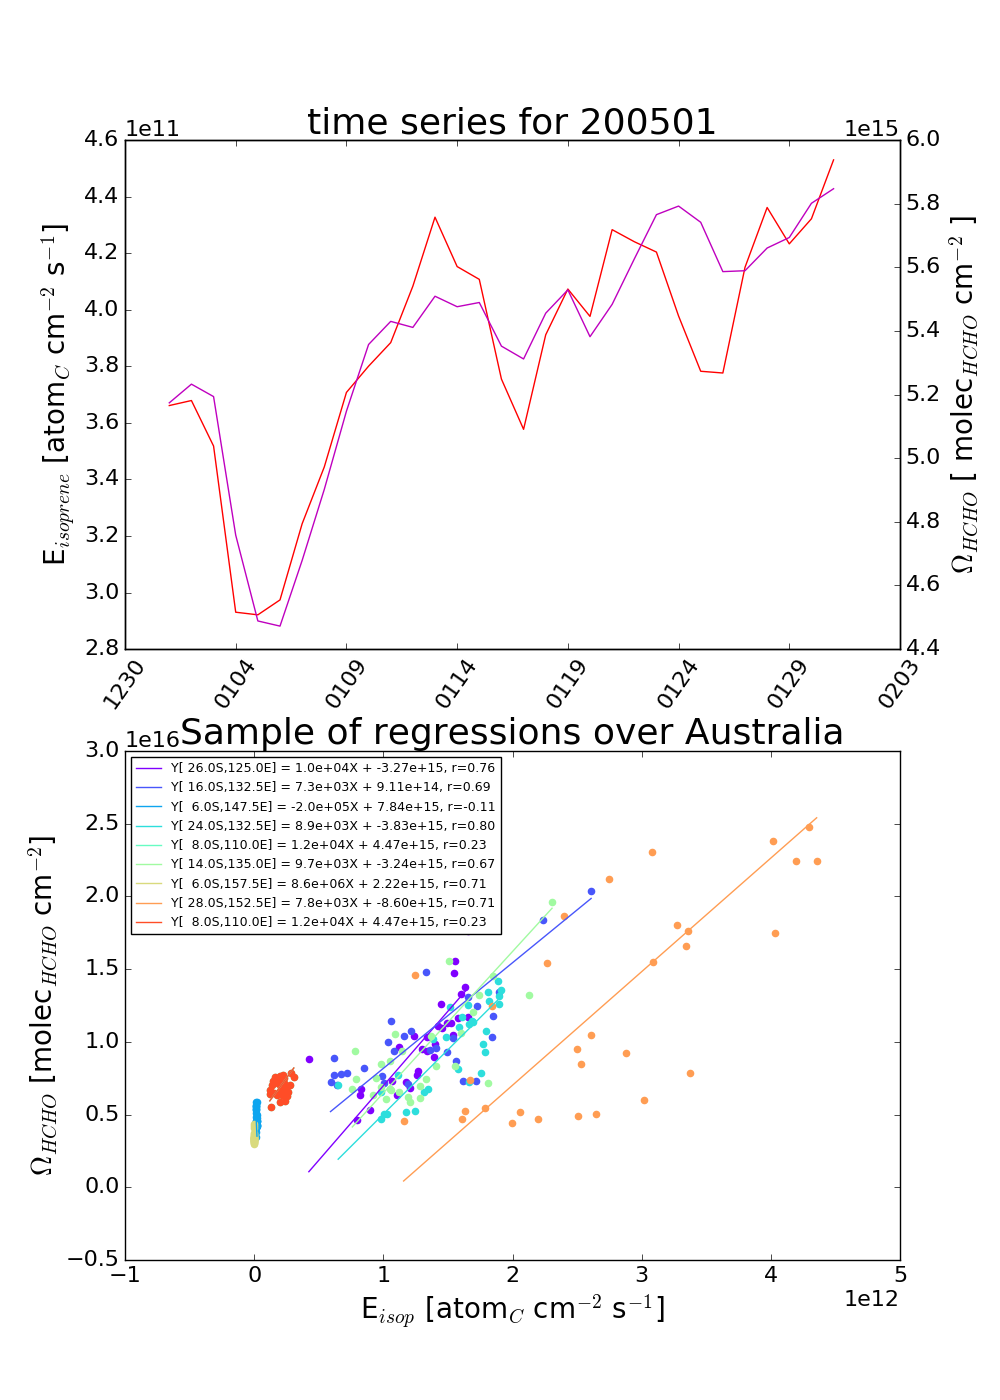
\includegraphics[width=\textwidth]{figures/E_isop_vs_hcho_series_200501.png}
      \caption{%
        Top panel: isoprene emissions for January, 2005, shown in red, coplotted with tropospheric hcho columns, shown in magenta.
        Both series are daily averages over Australia.
	      Bottom panel: (RMA) linear regressions from between emissions of isoprene and tropospheric hcho columns, sampled randomly from the 2$^{\circ}$ by 2.5$^{\circ}$ latitude longitude gridboxes over Australia for the month of January (2005).
      }
      \label{fig:E_isop_vs_hcho_model_sample}
    \end{figure}
    
    TODO: put this into results
    Using this modelled slope at 2$^{\circ}$ by 2.5$^{\circ}$ and applying it to equation \ref{eqn:isop_yield} with B and $\Omega_{HCHO}$ calculated using OMI satellite measurements provides a new estimate of isoprene emissions.
    Figure \ref{fig:E_isop_200501} shows the emissions calculated this way along with the Emissions output by GEOS-Chem averaged over January, 2005.
    \begin{figure}[!htbp]
      % Figure from Inversion.py -> check_against_MEGAN()
      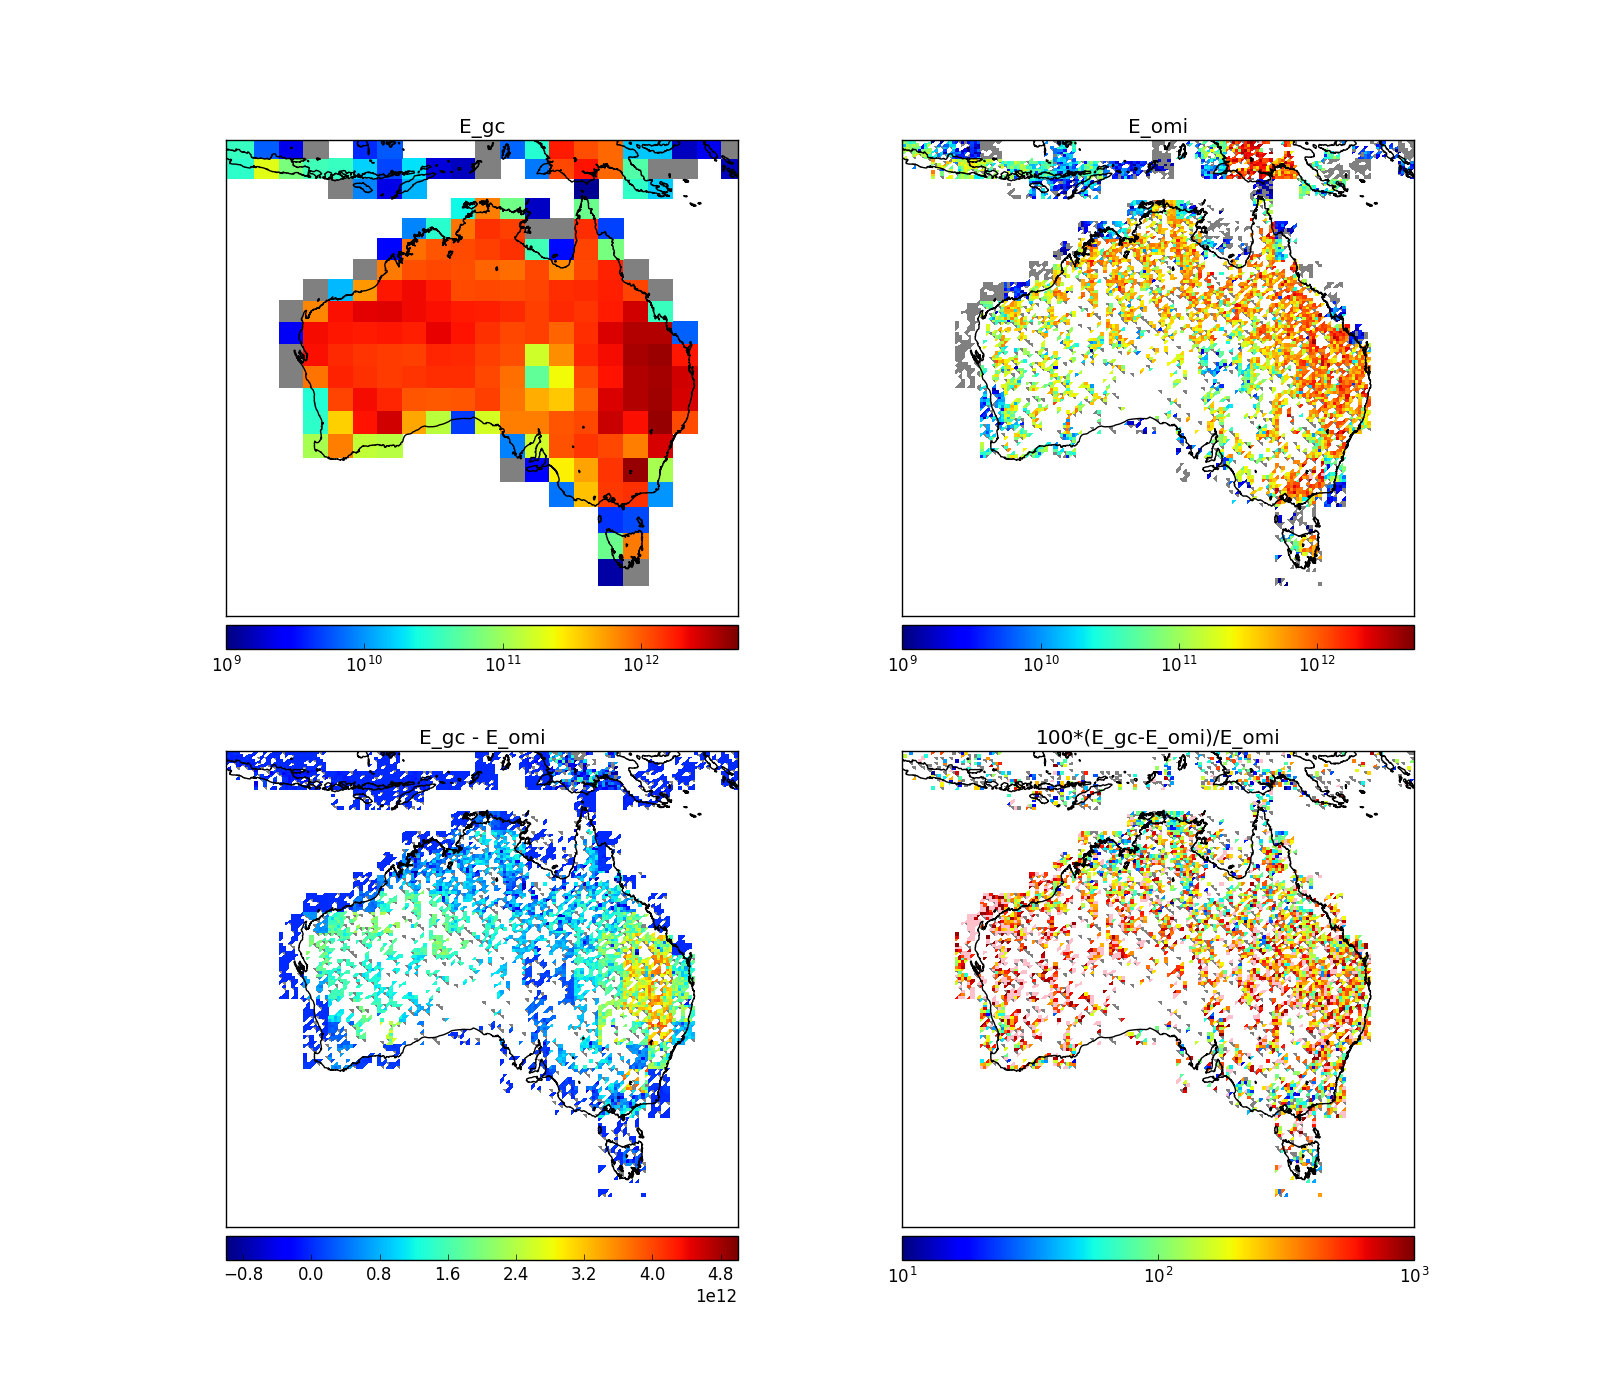
\includegraphics[width=\textwidth]{figures/E_Comparison.png}
      \caption{%
	Top row is isoprene emissions for the month of January, in 2005, from GEOS-Chem and estimated from OMI respectively.
	Bottom row shows the absolute and relative differences between the two.
      }
      \label{fig:E_isop_200501}
    \end{figure}
    
  \subsection{Emisions drivers}
    Calculated yields of HCHO can be classified using a box model which approximates specific environments.
    TODO: A table of different factors affecting emissions for three scenarios; urban, forest, shrublands is given in Table XX.
    The calculated yields for these scenarios is based on the CAABA/MECCA box model described in Section \ref{sec:CabbaMecca}TODO: compare scenarios yields and show map of Australia with mapped closest scenario(one colour for each scenario, contourf).
    
\section{Results}
  
  
  
  \subsection{Emissions affect on GEOS-Chem}
    We interpolated or something (TODO) the emissions over Australia into the inventories used by GEOS-Chem which reduced the emissions by X\% per year (over Australia).
    The resulting simulation output shows that HCHO was reduced by X\%, although if we boost monoterpenes by X\% where the isoprene emissions were lowered then 
    
  \subsection{Emissions comparisons}
    
    Some global numbers (TODO: where do I throw these?)
    \citet{Guenther2012} Estimate global biogenic isoprene emissions at roughly 535\tgpyr, using MEGAN.
    \citet{Sindelarova2014} Estimate around 594\tgpyr using MEGAN with MACC, showing isoprene as 69.2\% of the total BVOC emissions, with monoterpenes at 10.9\tgpyr (10.9\%).
    They show 41\tgpyr decrease in Australia when introducing soil moisture parameterisation.
    
    
    When comparing the GEOS-Chem (which runs MEGAN) emissions to those calculated using our top-down inversion, we see a decrease over TODO: locations and seasons.
    TODO: table or figure showing summary of isoprene emissions changes over the whole of our time domain.
    
    One set of data from the Daintree rainforest in Queensland exists (TODO: summary from P. Nelson).
    Although the data set lies outside our run times, as it was measured in TODO(runtime), we compare against the seasonal average of our GEOS-Chem output for the matching months (TODO: name the months).
    This is done for both GEOS-Chem output and our recalculated isoprene emissions.
    When compared against GEOS-Chem output we see TODO.
    When compared against recalculated emissions we see TODO.
    
    TODO: Figure showing campaign data against model and recalculated emissions over region for averaged months and eventually different resolutions.
    
    %As is done in \cite{Emmerson2016}, 
    We examine the affect of decreased isoprene emissions on the correlation between modelled and satellite based HCHO columns.
    Figure TODO: shows the regressions between GEOS-Chem tropospheric column amounts of HCHO and satellite columns for two runs of GEOS-Chem: a) using standard MEGAN emissions, b) using our updated emissions.
    
    
    
\conclusions  %% \conclusions[modified heading if necessary]


\appendix
% \section{}    %% Appendix A
% \subsection{}     %% Appendix A1, A2, etc.

\appendixfigures  %% needs to be added in front of appendix figures in one-column style (\documentclass[acp, manuscript]{copernicus})
\appendixtables   %% needs to be added in front of appendix tables in one-column style (\documentclass[acp, manuscript]{copernicus})

\authorcontribution{}

\competinginterests{The authors declare that they have no conflict of interest.}

%\disclaimer{disclaimer}

% Data availability
%
\textit{Data availability.} All GEOS-Chem model output is available from the authors upon request.

\begin{acknowledgements}
This research is supported by an Australian Government Research Training Program (RTP) Scholarship.
\end{acknowledgements}

%% Since the Copernicus LaTeX package includes the BibTeX style file copernicus.bst,
%% authors experienced with BibTeX only have to include the following two lines:
%%
\bibliographystyle{copernicus}
\bibliography{bibliography/hcho.bib}

\end{document}
